\documentclass{standalone}
\usepackage[dvipsnames]{xcolor}
\usepackage{tikz}
\usetikzlibrary{arrows.meta,matrix,positioning,fit}

\colorlet{2bit}{Melon}
\colorlet{4bit}{SkyBlue}
\colorlet{8bit}{LimeGreen}


\begin{document}

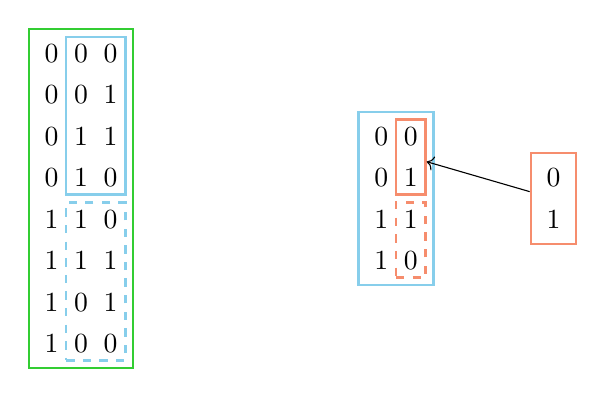
\begin{tikzpicture}[
  outline/.style={thick,inner sep=0mm},
  reversed/.style={dashed},
  graytable/.style={
    outline,
    matrix of nodes,
    draw,
    nodes={color=black,minimum height=0,outer sep=0},
    column sep=0,
    row sep=1mm,
    inner sep=1mm
  }
]
\matrix (G8) [graytable,color=8bit] at (0,1)
{
  0&0&0\\
  0&0&1\\
  0&1&1\\
  0&1&0\\
  1&1&0\\
  1&1&1\\
  1&0&1\\
  1&0&0\\
};
\matrix (G4) [graytable,color=4bit] at (4, 1)
{
  0&0\\
  0&1\\
  1&1\\
  1&0\\
};
\matrix (G2) [graytable,color=2bit] at (6,1)
{
  0\\
  1\\
};

\node[outline,fit={(G4-1-2.north west) (G4-2-2.south east)},draw=2bit] (G2emb){};
\node[outline,reversed,fit={(G4-3-2.north west) (G4-4-2.south east)},draw=2bit]{};

\node[outline,fit={(G8-1-2.north west) (G8-4-3.south east)},draw=4bit]{};
\node[outline,reversed,fit={(G8-5-2.north west) (G8-8-3.south east)},draw=4bit]{};

\draw[->]  (G2) -- (G2emb);

\end{tikzpicture}

\end{document}
